%%
%%  Example paper
%%
%%

%%%%%%%%%%%%%%%%%% Usenix style %%%%%%%%%%%%%%%%%%%%%%%%%%%%%%%%%
\documentclass[10pt,twocolumn,a4paper]{article}
\usepackage{styles/usenix-style}

\author{Fabian Nguyen}

%%%%%%%%%%%%%%%%%% Document %%%%%%%%%%%%%%%%%%%%%%%%%%%%%%%%%%%%%%%%%%%
% TODO: Change draft to final before submitting final version.
\usepackage[draft]{styles/ka-style}
\usepackage{cite,xspace,ifthen,graphicx,listings}
\usepackage[font=small,labelfont=bf]{caption}
\usepackage[
   pdfauthor={Fabian Nguyen},
   pdftitle={Advanced Exploit Mitigation},
   pdfsubject={Windows Internals},
   pdfkeywords={Security,Stack Overflow,Return Oriented Programming, Control Flow Guard, Shadow Stack}
]{hyperref}

\begin{document}

\title{ Windows Internals: Advanced Exploit Mitigation }

\newcommand{\todo}[1]{{\texttt{[#1]}}}
\newcommand{\code}[1]{{\tt \small{#1}}}

\maketitle
%\draftfooter

\begin{abstract}
We take a look at general techniques used by attackers to compromise Windows systems and some fundamental defense mechanisms against them.
This paper will provide an overview of Microsoft's latest additions to the security concept of the Windows Operating System [OS] , analyze inherent flaws in their design and take a brief look at already existing attacks. 
\end{abstract}

\section{Introduction}\label{sec:introduction}
In an increasingly digitalized world an overwhelming amount of private and/or safety-critical information and data is stored on computers.
Windows is by far the most used operating system and therefore the main target of attackers to compromise data or computer systems.
One common intent of attackers is to steal an individual's passcode for a website, e.g an online-banking website.
Naturally, as the amount and complexity of attacks rises, OS vendors are forced to put an increasingly high amount of effort into mitigating existing weaknesses and deny attackers of further possibilities to compromise their OS.
Even though this is the case, the amount of potentially abusable vulnerabilities in Windows has been increasing, instead of decreasing.
\citeonline{CVE}

\begin{figure}[htbp]
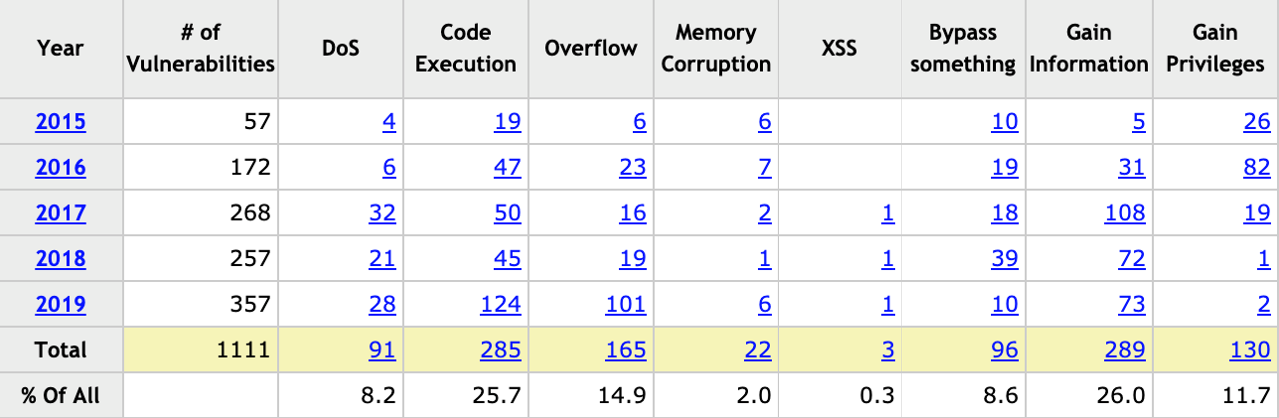
\includegraphics[width=8cm, height=2.5cm]{fig/stats}
\caption{Amount of documented vulnerabilities in the Windows Operating System.\newline Note that the spike in "Gain Information" vulnerabilities in 2017 is inflated by a family of attacks widely known as Meltdown/Spectre}
\end{figure}

We can see that the three largest groups of vulnerabilities consist of "Gain Information", "Code Execution" and "Overflow".
Of course these three categories aren't entirely seperated from each other.
An attacker that is able to execute Code on a machine often does so in order to gain information and overflows are often the reason why an attacker can execute code in the first place.
\section{Overflows}\label{sec:Overflows}
An overflow happens when a program writes data to memory beyond the limits of the intended data structure.
One common example of this is a stack buffer overflow caused by an incorrect use of the function \emph{strcpy}.More precisely, an overflow can occur when the given input is longer than the buffer one writes too.
%%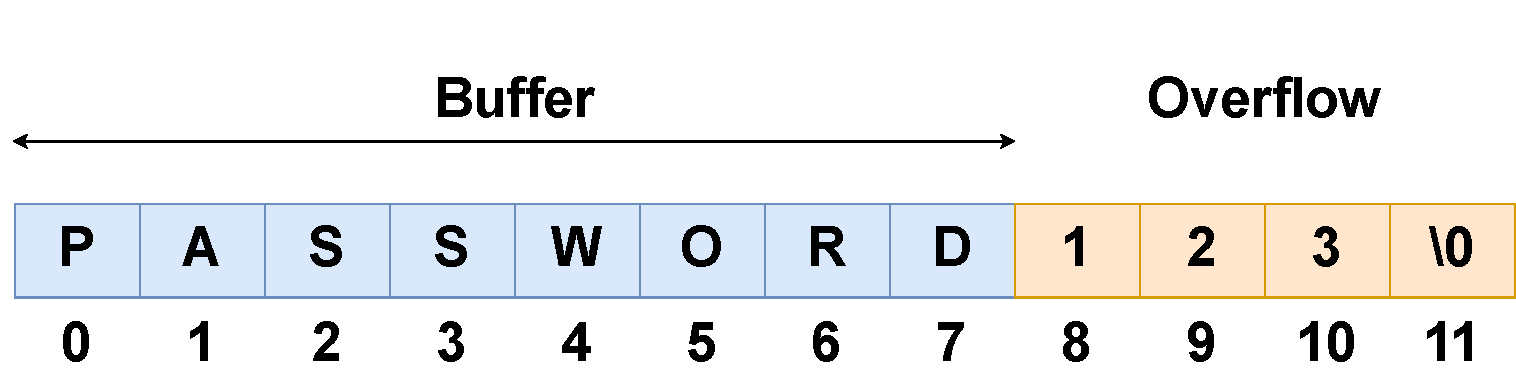
\includegraphics{fig/simpleoverflow}
%%\caption{The password's length is too large to fit into the designated buffer.However, strcpy will not check for valid sizes so it will continuously write beyond the buffer.}
Relatively small in size overflows like this in particular are not always easy to spot and often remain unidentified if they don't cause immediate errors.
Besides causing faulty program behaviour, this also provides a critical attack surface.
To see why this is the case, let's take a look at a typical stack buffer layout with only one buffer present right at the beginning.
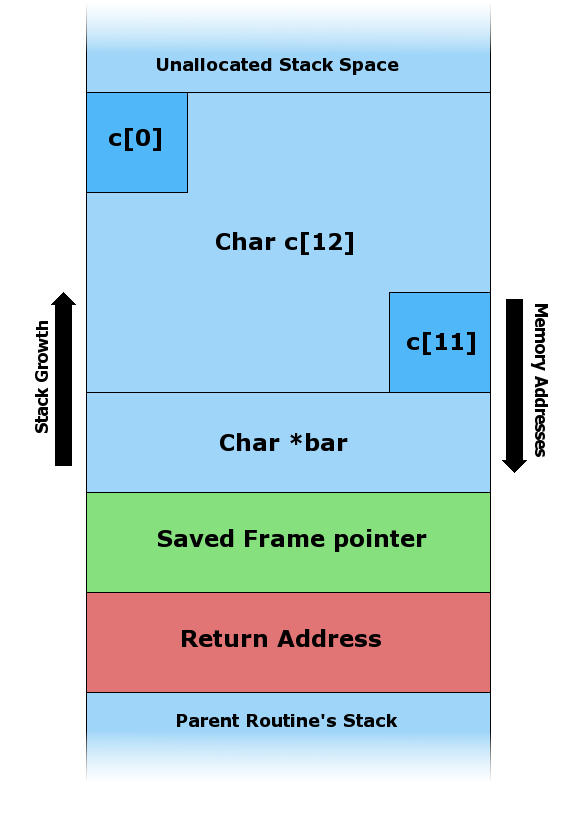
\includegraphics[height=8cm,width=7cm]{fig/Stack_Overflow}
\newline As we can see, the stack will usually contain a return adress right at the bottom, a frame pointer on top of it and then local data that is used by the current function. Obviously, one will also need to keep the parent function's data saved below (stack grows upwards).
In our example there is only one character buffer of size 12 and a pointer to it present.
\newline Suppose one wants to copy user-input string into this buffer, e.g by using strcpy.
The user may now unknowingly or perhaps purposely overflow this buffer by entering a string thats longer than 12 characters.
As we observed earlier, this will result in the memory after the buffer being written. Note that data is written from top to bottom.
\begin{figure}
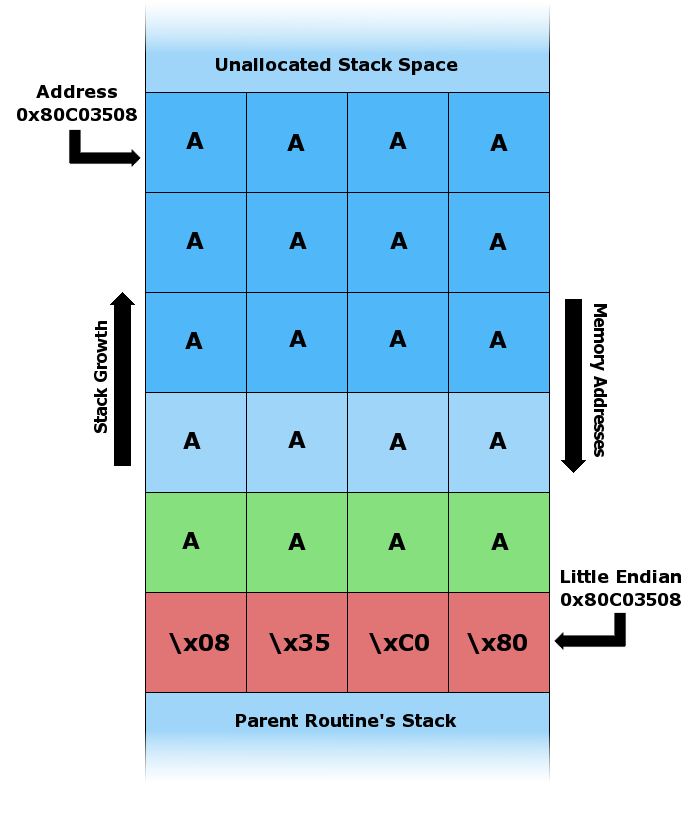
\includegraphics[height=8cm,width=8cm]{fig/Stack_Overflow2}
\caption{The user-input is too long for the given buffer}
\end{figure}
We see that our pointer to the buffer is overwritten, as well as the stack frame we had saved on the stack earlier. Most importantly though, the return adress is also corrupted.
In the given figure, the input is constructed so that the part that's written over the return adress resembles an adress itself. In this case, its just the adress of the buffer again.
At some point, our given function will attempt to return to this adress. However, once it does so, all it will be able to read from this adress is a swarm of  'A's which certainly doesnt resemble a valid sequence of code. The programm will fault and terminate.

 %\begin{figure}[htbp]
%  \centering
%  \fbox{\parbox{.8\columnwidth}{
%      Here you can include a sample figure.  Use something like
%      \begin{center}
%        \code{$\backslash$includegraphics[scale=.8]\{template\}}
%      \end{center}
%      to include an encapsulated postscript figure.  The \emph{scale}
%      argument can be used for scaling the picture, although it
%      may scale the font incorrectly.
%    }}
%  \caption{Sample Figure}
%  \label{fig:sample}
%\end{figure}


%\lstset{language=C, basicstyle=\ttfamily,
%        string=[b]', showspaces=false, showtabs=false,
%        caption={A sample code snippet}, captionpos=b}
%\begin{lstlisting}
%/* code snippet  */
%while (!sleep)
%	sleep++;
%\end{lstlisting}

%\begin{figure}[hbt]
%\centering
%\includegraphics[scale=.7,clip]{fig/OIUKAvV}
%\caption{Sample figure automatically from Windows prn.\label{plot:fig}}
%\end{figure}

\section{Related Work}\label{sec:relwork} 

\section{Approach}

\section{Conclusion}\label{sec:conclusion}

\bibliographystyle{abbrv}
\bibliography{Advanced Exploit Mitigation}
%\footnotesize
\end{document}
